\documentclass[12pt]{article}
\usepackage[hidelinks]{hyperref}    
\usepackage[all]{hypcap}   
\usepackage{graphicx}
\usepackage{amsmath}
\usepackage{listings}
\usepackage{xcolor}
\usepackage{float}

% Define custom settings for HACK assembly language
\lstdefinelanguage
    [HACK]{Assembler}
    {morekeywords={@SP, @LCL, @ARG, @THIS, @THAT, @SCREEN, @KBD}, % Common HACK symbols
     alsoother={=,;,@},  % Symbols used in HACK assembly
     sensitive=true,     % Case-sensitive
     morecomment=[l]//,  % Define comments to start with "//"
    }

% Set up the listing style for HACK assembly
\lstset{
    language=[HACK]Assembler,
    basicstyle=\ttfamily\small,      % Small monospace font
    keywordstyle=\color{blue},       % Keywords in blue
    commentstyle=\color{gray},       % Comments in gray
    stringstyle=\color{red},         % Strings in red
    tabsize=4,
    showstringspaces=false,
    numbers=left,                    % Line numbers on the left
    numberstyle=\tiny\color{gray},
    breaklines=true,
    frame=single,                    % Frame around the code
}
\graphicspath{{../images/}}
\author{Andrea Malvezzi}
\title{\textbf{Architettura degli Elaboratori\\ Pratica}}
\date{Novembre 2024 - $\dots$}
\author{Andrea Malvezzi}
\begin{document}
\maketitle
\pagebreak
\tableofcontents
\pagebreak

\section{Che cos'è l'ISA}
\label{sec:whats_ISA}
L'ISA è l'interfaccia tra HW e SW.
Costituisce il set di istruzioni con cui opera la CPU e di conseguenza, varia di architettura in architettura.

\section{L'architettura HACK}
\label{sec:HACK_architecture}
L'architettura HACK non segue né la filosofia CISC né quella RISC e, data la sua semplicità, in essa ad ogni istruzione eseguita corrisponde un ciclo di clock.
Qui si usano una RAM (per contenere i dati di un programma in esecuzione) e una ROM (per contenere il programma \textit{stesso}) a 16 bit. \\
Si utilizzano prevalentemente tre registri di memoria: \textbf{A}, \textbf{D} ed \textbf{M}.
\\Il registro M è particolare, in quanto contiene il valore del registro di memoria RAM attualmente puntato da A. Questo si indica con RAM[A]. \\
Oltre a questi due si usa inoltre il \textbf{Program Counter}, o \textbf{PC}. In esso è contenuto l'indirizzo della prossima istruzione da eseguire e si indica con ROM[PC].

\section{Tipi di istruzione}
\label{sec:tipi_istruzione}
Esistono due tipi di istruzioni:
\begin{itemize}
    \item A-instruction: quelle che lavorano sulla memoria (che caricano valori in A);
    \item C-instruction: quelle che eseguono un instruzione (sfruttando l'ALU) prelevando gli operandi dai registri A,D ed M.
\end{itemize}
Le C-instruction solitamente seguono la forma generale $\text{dest} = \text{comp}; \text{jump}$, dove:
\begin{itemize}
    \item \textbf{dest}: opzionale. Specifica dove memorizzare il risultato\\dell'operazione;
    \item \textbf{comp}: specifica l'operazione da eseguire;
    \item \textbf{jump}: opzionale. Specifica se, dopo aver eseguito $\text{dest} = \text{comp}$ occorre fare un salto nel programma alla linea specificata dal valore del registro A (esegue $\text{PC} = A)$. Funziona effettivamente come un \textit{if} eseguito sempre rispetto allo zero. 
\end{itemize}

\subsection{Tutte le possibili operazioni}
\label{ssec:operazioni_possibili}
A seguire tutte le possibili operazioni eseguibili nell'architettura HACK.
\begin{figure}[!htb]
    \centering
    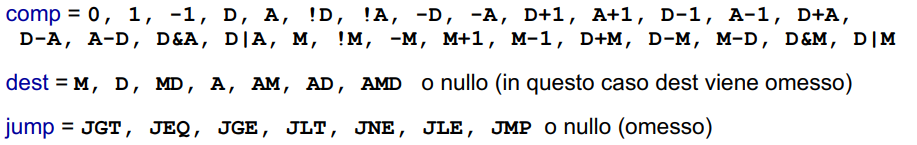
\includegraphics[width=.9\linewidth,height=.40\textheight,keepaspectratio]{ISA_HACK/operazioni.png} % essenzialmente resiza l'immagine
    \begin{center}
        \caption{\label{fig:operazioni} Se un'operazione che si desidera eseguire non compare qui, allora occorre cambiare approcio.} % label fuori da caption spesso non va, mettilo dentro
    \end{center}
\end{figure}
\subsubsection{Esempio di operazione}
\label{sssec:operazioni_esempi}
\begin{gather*}
    @2\\
    \text{D}=\text{D} + 1;\text{JLT}
\end{gather*}
Questa riga di codice aumenta di 1 il valore del registro D, poi controlla che questo valore sia strettamente minore di 0.
Nel caso in cui questa condizione risultasse verificata, verrà effettuato un JUMP alla riga corrispondente al valore corrente di A, quindi, alla seconda.

\section{Le etichette}
\label{sec:etichette}
Un'etichetta è un'istruzione composta di due parti: quella di dichiarazione e quella di chiamata.

\subsection{Dichiarazione di etichetta}
\label{ssec:dichiarazione_etichetta}
Un'etichetta fornisce un modo per non dover scrivere a mano (e quindi commettere errori) ogni A-instruction prima di effettuare un salto.
Difatti, l'etichetta prende il valore del numero di riga in cui viene dichiarata, permettendo poi di saltare a quella eventuale riga qualora risultasse necessario.
\subsubsection{Esempio di dichiarazione di etichetta}
\label{sssec:esempio_dichiarazione_etichetta}
\begin{gather*}
    (\text{MIA\_ETICHETTA})\\
    \dots \text{codice} \dots
\end{gather*}
Qui l'etichetta viene definita prima di un blocco di codice e prende il nome di MIA\_ETICHETTA.
Questa etichetta avrà quindi ora il valore della riga a cui è stata dichiarata (quella prima del blocco di codice).

\subsection{Utilizzo dell'etichetta}
\label{ssec:utilizzo_etichetta}
Questa etichetta contiene ora il numero della riga in cui è stata dichiarata e, in quanto tale, fornisce un modo per saltare a tale riga mediante una istruzione JUMP.
\subsubsection{Esempio di utilizzo dell'etichetta}
\label{sssec:esempio_utilizzo_etichetta}
\begin{gather*}
    @\text{MIA\_ETICHETTA}\\
    0;\text{JMP}
\end{gather*}
Questo ci permette di assegnare ad A il valore della riga in cui l'etichetta è stata dichiarata, per poi eseguire un salto incondizionato (0 è sempre zero, quindi il JMP verrà sempre effettuato) alla riga corrispondente all'inizio del blocco di codice sottostante all'etichetta.
\pagebreak

\section{Costrutti della programmazione}
\label{sec:costrutti_programmazione}

\subsection{If-then-else}
\label{ssec:if_then_else}
Si può ricreare il costrutto if-then-else tramite JUMP, A/C-instruction ed etichette.
\begin{lstlisting}
    // Costrutto if-then-else
    D=1             // Dato da testare

    @CASE_FALSE     // A=riga del caso false
    D;JLE           // Se D <= 0, JUMP al valore di A

    // Se salto, questo blocco non viene eseguito
    ...caso true... 

    @END            // A=riga fine codice
    0;JMP           // Salto incondizionato

    (CASE_FALSE)    // Dichiaro l'etichetta
    ...caso false...

    (END)           // Dichiaro l'etichetta
    ...fine codice...
\end{lstlisting}

\pagebreak
\subsection{Ciclo while}
\label{ssec:while}
Anche il ciclo while si può ricreare mediante JUMP, A/C-instruction ed etichette, seppure in maniera leggermente più complessa.
\begin{lstlisting}
    // Ciclo while
    D=10             // Variabile per iterazione

    (LOOP)          // Dichiaro inizio loop
    D; JLE          // JMP se D<=0
    
    ...codice...    // Se salto, questo viene saltato

    @LOOP           // Al termine del codice, rifai
    0;JMP           // Salto incondizionato

    (EXIT)          // Dichiaro uscita loop
    ...altro codice...
\end{lstlisting}

\pagebreak
\section{Cose a cui prestare attenzione}
\label{sec:nb_1}

\subsection{Fine dei programmi}
\label{ssec:fine_programma}
Di base i programmi non finiscono, ma continuano ad incrementare il PC fino a che non si esaurisce la ROM.
Per evitare questa behaviour, è buona pratica terminare un programma con un ciclo dummy che previene quindi di andare ad eseguire istruzioni scritte nelle celle della ROM successive.
\begin{lstlisting}
    // Ciclo dummy
    ...codice programma...
    
    // Dichiaro un ciclo infinito
    (END)       // Dichiaro fine programma
        @END    // A=Riga precedente
        0;JMP   // Salto incondizionato
\end{lstlisting}

\subsection{Comparazioni tra valori diversi da 0}
\label{ssec:compare_values}
Come visto in precedenza, esistono solo comparazioni rispetto lo 0. Per ovviare a questa limitazione, si possono usare la somma e la sottrazione.
\begin{lstlisting}
    // A <= 10?
    @2      // A=2
    D=10    // D=10
    D=D-A   // D=D-A, quindi D=10-2

    @ELSE   // Preparo A per saltare all'else case
    D:JLE   // Se D<=0, JUMP

    ...caso true...
    @END    // Termina programma
    0;JMP   // Salto incondizionato

    (ELSE)  // Dichiaro else case
        ...caso false...

    (END)   // Dichiaro ciclo dummy finale
        @END
        0;JMP
\end{lstlisting}

\section{Le variabili}
\label{sec:variables}
Anche in asm HACK si hanno le variabili, anche se funzionano in modo leggermente diverso.
Qui si definiscono come A-instruction e si va a modificare il valore interno al loro registro.
\begin{lstlisting}
    // Esempio di uso delle variabili
    @i          // Variabile i
    M=1         // Registro di i pari ad 1 (RAM[i]=1)

    (LOOP)      // Dichiaro inizio loop
        @i      // uso i
        D=M     // D=Valore registro di i
        @10     // A=10
        D=D-A   // D=D-A, quindi D=i-10

        @END    // Preparo a terminare il programma
        D;JGT   // Se D>0, JUMP

        ...codice loop...
        @i      // Uso i
        M=M+1   // Aumento di 1 il valore di RAM[i]
        ...codice loop...

        @LOOP   // Preparo per ricominciare
        0;JMP   // Salto incondizionato
    
        (END)   // Dichiaro ciclo dummy finale
            @END
            0;JMP
        
        // La variabile i serve ad iterare nel loop
        // fino a quando non equivale ad 11 (i-10>10)
\end{lstlisting}
Esistono inoltre variabili pre-definite per accedere in maniera più esplicita alla memoria RAM, come @R\textit{n}, dove \textit{n} va da 0 a 15. 
\pagebreak
\section{Cose a cui prestare attenzione}
\label{sec:nb_2}

\subsection{Naming conventions}
\label{ssec:nb_naming_conventions}
Generalmente le variabili hanno nomi in minuscolo, mentre le etichette in maiuscolo.

\subsection{Nota sull'uso delle variabili}
\label{ssec:nb_using_variables}
In termini pratici, i primi 16 indirizzi della memoria RAM (da @R0 a @R15) sono riservati per l'esecuzione del programma in esecuzione.
Tutti gli indirizzi successivi saranno utilizzati da eventuali variabili, a scelta dell'assemblatore. \\
Per questo motivo, qualora in un programma ci si ritrovasse a dover scrivere qualcosa come @16 oppure un qualunque valore superiore a 15, allora non si dovranno utilizzare variabili, in quanto queste rischierebbero di essere sovrascritte.

\section{Il computer HACK}
\label{sec:premises}
Il computer HACK sfrutta l'architettura Von Neumann a 16-bit, con una feature di quella Harvard:
la memoria dati viene separata da quella programma, in modo da poter caricare contemporaneamente dati e istruzioni.
\\
Questo viene reso possibile dal bus dati che, mentre nelle architetture moderne svolge due compiti distinti e quindi non eseguibili in parallelo, qui ne svolge solamente uno.
Conseguentemente per eseguire un'istruzione basta un ciclo di clock.

\section{La memoria}
\label{sec:memory}

\subsection{La ROM}
\label{ssec:ROM}
La ROM corrisponde ad un chip built-in che dato un address 15-bit codifica in binario
un'istruzione da eseguire, quindi: $\text{out} = \text{ROM}32\text{K}[address]$.

\subsection{Chip memory}
\label{ssec:memory_chip}
Il chip memory è composto da un totale di 3 componenti, per un totale di 24K indirizzi:
\begin{itemize}
    \item la RAM da 16K;
    \item il chip \textbf{Screen} da 8K, usato per mappare lo schermo;
    \item un singolo registro \textbf{Keyboard} per leggere il tasto premuto;
\end{itemize} 
Tuttavia, avendo in ingresso un address da 15 bit da convertire in binario, si sprecano molti indirizzi così facendo: $2^{15}=32767$ meno i 24576 occupati dal chip memory, per un totale di 8191 indirizzi sprecati. Cosa accade a questi?

\subsubsection{Il chip Screen}
\label{sssec:screen_chip}
All'interno del chip Screen si ha una corrispondenza diretta tra il singolo bit e un pixel sullo schermo. In base al valore di questi bit, lo schermo viene costsantemente refreshato colorando di bianco (0) o di nero (1) ogni singolo pixel.
\\
Per impostare il pixel in posizione (row, col) dello schermo ad un certo colore, occorrerà quindi settare il bit $col\%16$ della word all'indirizzo Screen[row*32 + col/16] a 1 oppure a 0.
\\
Ma come mai questi numeri? Anzitutto, occorre specificare che nel computer HACK lo schermo è composto da 256 righe e 512 colonne.
\\
Questo significa che in una singola riga ci saranno 512 caratteri, raggruppati in parole (che in informatica hanno spesso una grandezza di 16 bit),
da cui si evince che in una singola riga si avranno 32 parole ($512/16=32$). Ed ecco spiegato il \textbf{row*32}.
\\
Lo stesso ragionamento va applicato alle righe: avendo 256 righe, si avranno 16 ($256/16=16$) parole per colonna, da cui \textbf{col/16}.

\subsubsection{Esempio di codice per disegnare un rettangolo largo 16 pixel e alto MEM[0] pixel}
\label{sssec:rectangle_example}
\begin{lstlisting}
    @0              // A=0
    D=M             // D=RAM[0]

    @INFINITE_LOOP  // Preparo il salto
    D; JGE          // Se D>0

    @counter        // Variabile counter per iterare
    M=D             // RAM[counter]=RAM[0]

    @SCREEN         // Predefinita dal linguaggio
    D=A             // D=Indirizzo Screen
    @address        // Variabile address
    M=D             // RAM[address]=Indirizzo Screen

    (LOOP)
        @address    // Variabile address
        A=M         // A=Indirizzo Screen
        M=-1        // MEM[Indirizzo Screen]=-1
        
        @32         // A=32
        D=A         // D=32
        @address    // Variabile address
        M=M+D       // Address+=32

        @counter
        MD=M-1      // Counter--, D per check sul jump

        @LOOP       
        D;JGT       // Torno all'inizio

    (END)           // Ciclo dummy finale
        @END
        0;JMP
\end{lstlisting}

\subsubsection{Il chip Keyboard}
\label{sssec:keyboard_chip}
Come annunciato precedentemente questo chip è composto da un solo registro e fornisce in output la codifica ASCII estesa del tasto premuto, oppure 0 se non si preme alcun tasto.
\\
Il registro è read-only e vi sono alcuni tasti con codifiche particolari, come lo spazio.

\section{Comportamento della CPU}
\label{sec:CPU}
\begin{figure}[H]
    \centering
    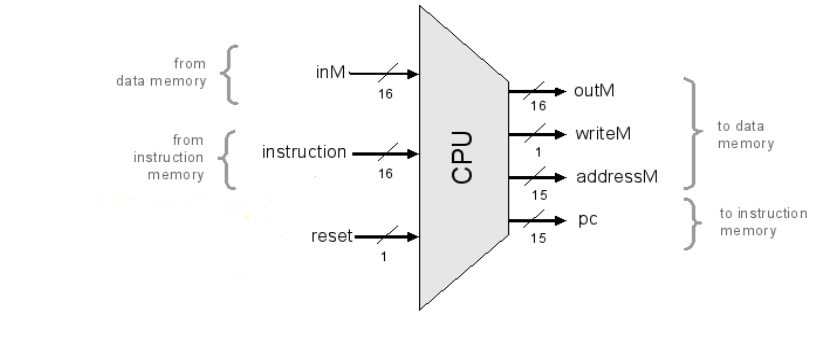
\includegraphics[width=1\textwidth, height=.7\textheight,keepaspectratio]{realizzare_HACK/CPU.png} % essenzialmente resiza l'immagine
    \begin{center}
        \caption{\label{fig:come_funziona_CPU}Schema logico CPU nell'architettura HACK.} % label fuori da caption spesso non va, mettilo dentro
    \end{center}
\end{figure}
La CPU è composta da 4 componenti: l'ALU e 3 registri, quali A, D, PC.
Questa esegue istruzioni seguendo le specifiche del linguaggio HACK (nel nostro caso). Ovvero:
\begin{itemize}
    \item i valori D ed A, se presenti, sono letti e/o scritti nei registri A ed M;
    \item il valore M, se presente nella right side dell'istruzione da eseguire, viene LETTO da inM (input-M);
    \item se invece il valore M risulta presente nella left side dell'istruzione da eseguire, allora
            l'output verrà scritto in outM, A prenderà il valore di addressM e writeM verrà alzato ad 1.
\end{itemize}

\section{Codifica A-Instruction}
\label{sec:A-instruction}
In HACK le A-instruction sono codificate nella maniera seguente: il bit di segno (o modulo) è sempre pari a 0, mentre i 15 valori a seguire saranno cifre binarie.
\begin{figure}[H]
    \centering
    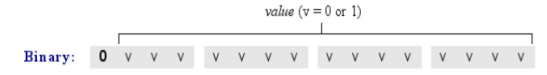
\includegraphics[width=1\textwidth, height=.7\textheight,keepaspectratio]{realizzare_HACK/a_instruction.png} % essenzialmente resiza l'immagine
    \begin{center}
        \caption{\label{fig:codifica_a_instruction}Codifica delle A-instruction nell'architettura HACK.} % label fuori da caption spesso non va, mettilo dentro
    \end{center}
\end{figure}
Tramite questo approcio si possono codificare tutti i valori non negativi codificabili in complemento a 2 con 16 bit (si ha effettivamente un bit in meno, quello modulo).

\section{Codifica C-instruction}
\label{sec:C-instruction}
Nell'architettura HACK le C-instruction sono codificate nella maniera
\\
seguente: il modulo e le due cifre subito dopo di esso sono \textbf{sempre} pari ad 1, ed i valori seguenti sono posti ad 1 solamente quando alcune caratteristiche vengono rispettate.
\begin{figure}[H]
    \centering
    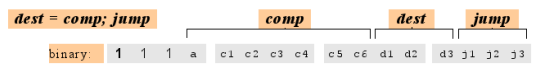
\includegraphics[width=1\textwidth, height=.7\textheight,keepaspectratio]{realizzare_HACK/c_instruction.png} % essenzialmente resiza l'immagine
    \begin{center}
        \caption{\label{fig:codifica_c_instruction}Codifica delle C-instruction nell'architettura HACK.} % label fuori da caption spesso non va, mettilo dentro
    \end{center}
\end{figure}

E come possibile vedere dalla figura, il corpo effettivo dell'istruzione è composto da valori impostati a seconda della presenza di alcune direttive. Ma come sono decisi questi valori? tramite la seguente tabella:
\begin{figure}[H]
    \centering
    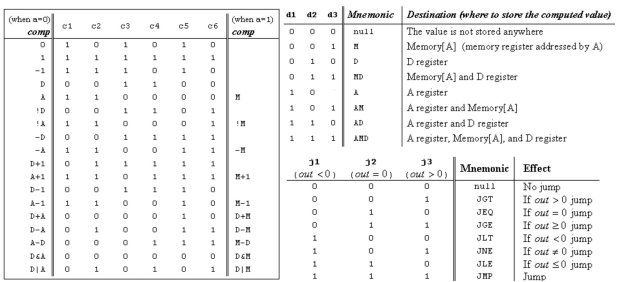
\includegraphics[width=1\textwidth, height=.7\textheight,keepaspectratio]{realizzare_HACK/tabella_c_instruction.png} % essenzialmente resiza l'immagine
    \begin{center}
        \caption{\label{fig:c_instruction_tabella}Ad esempio un'istruzione contenente un JGT avrebbe gli ultimi 3 bit (quelli di \textit{jump}) pari a $001$.} % label fuori da caption spesso non va, mettilo dentro
    \end{center}
\end{figure}

\section{Che cos'è l'Assembler}
\label{sec:whats_assembler}
L'assembler si occupa di tradurre da linguaggio Assembly a binario il nostro codice. Si passa quindi da istruzioni, etichette e simboli speciali a sequenze di 16 bit, generando in output un file \textit{.hack}.
\\
Oltre a quanto citato, l'assembler si occupa anche di tradurre spazi, righe vuote e simboli come \textit{\textbackslash{n}} o \textit{\textbackslash{t}} (ignorando quindi i commenti).

\section{Traduzione di A-instructions}
\label{sec:a_instructions_translation_details}
Ricordando la traduzione delle A-instructions spiegata precedentemente,
\\
basta porre il primo bit della sequenza a 0 e poi tradurre il numero specificato nel codice. Ad esempio:
\[ @3 \Rightarrow \textcolor{red}{0}00000000000011 \]

\section{Traduzione di C-instructions}
\label{sec:c_instructions_translation_details}
Non occorre imparare a memoria la tabella, ma bensì conoscere a grandi linee il significato di una traduzione in bit, qualora se ne trovasse una. Ad esempio:
\[ D=A \Rightarrow \textcolor{red}{111}0\textcolor{blue}{0110000}\textcolor{yellow}{010}\textcolor{green}{000} \]
Dove le cifre in rosso sono valori fissi delle C-instructions.
\\
Quelli in blue sono le istruzioni inerenti alla \textit{comp}, ovvero l'istruzione effettiva da eseguire (in questo caso A), con davanti il valore di a (qui è 0).
\\
Quella gialla sono la parte \textit{comp}, ovvero la destinazione dove salvare il risultato dell'operazione (nel nostro caso D).
\\
La parte verde è la sezione per il \textit{jump}. Ovviamente, non avendo un jump, ogni bit sarà posto a 0.

\section{Gestione dei simboli}
\label{sec:gestione_simboli}
I simboli si usano per identificare certi indirizzi nella ROM (destinazione salti) o nella RAM (dove son contenute le variabili).
\\
Alcuni simboli potrebbero essere le lettere, le cifre o caratteri speciali come \_,-,. etc $\dots$
L'unica accortezza consiste nel non scrivere una cifra all'inizio di un simbolo (ed ecco spiegato perché non si può cominciare il nome di una variabile con un numero).

\subsection{Simboli predefiniti}
\label{ssec:simboli_predef}
Alcuni simboli sono pre-esistenti nel linguaggio, ovvero $\dots$
\begin{itemize}
    \item $\dots$ I registri virtuali: I simboli da R0 a R15 fanno riferimento agli indirizzi RAM da 0 a 15;
    \item $\dots$ I puntatori per I/O: I simboli SCREEN e KBD fanno riferimento rispettivamente agli indirizzi RAM 16384 e 24576;
    \item $\dots$ I puntatori di controllo della VM: I simboli SP, LCL, ARG, THIS e THAT fanno riferimento agli indirizzi RAM da 0 a 4, rispettivamente.
\end{itemize}

\subsection{Simboli NON predefiniti}
\label{ssec:simboli_non_predef}
Ci sono poi anche simboli non definiti dal linguaggi, ovvero le etichette e le variabili.
\\
Le prime sono usate per identificare la destinazione dei JUMP e a queste è assegnato come valore l'indirizzo della ROM in cui verrà caricata la prossima istruzione da eseguire. Ad esempio:
\begin{lstlisting}
    // Valore: numero della riga contenente
    // l'istruzione seguente
    (LOOP)
        istruzione 1...
        istruzione 2...
        istruzione 3...
\end{lstlisting}
Le seconde sono usate nelle A-instructions per identificare celle della memoria RAM a partire dalla 16-esima. Riceveranno quindi un valore che va dal 16 in poi. Ad esempio:
\begin{lstlisting}
    @counter        // Valore: 16
    ...codice...
    @max            // Valore: 17
    ...codice...
    @min            // Valore: 18
    ...codice...
\end{lstlisting}

\section{Procedura di assemblaggio}
\label{sec:proc_assemblaggio}
Il processo di assemblaggio è diviso in 3 fasi:

\subsection{Inizializzazione}
\label{ssec:proc_init}
\begin{itemize}
    \item si apre in lettura il file .asm in input;
    \item si inizializza la symbol table dei simboli predefiniti;
\end{itemize}

\subsection{Prima passata}
\label{proc_first}
Si scorre l'input per inserire nella symbol table le codifiche delle etichette incontrate.
Per farlo si usa un counter del totale delle A/C-instructions incontrate, assegnando a ogni etichetta il valore corrente del counter +1.

\subsection{Seconda passata}
\label{proc_second}
Si apre in writing il file .hack prodotto e si scorre nuovamente l'input.
Per ogni A/C-instruction incontrata ne si scrive nell'out la relativa codifica.
Inoltre qualora una A-instruction usasse un simbolo, si dovrebbe ricercare questo nella symbol table e, nel caso in cui questo sia assente (quindi si sta parlando di una variabile) si assegna a questa istruzione un valore progressivo a partire da 16, per poi memorizzare questo nella symbol table. 

\subsection{Esempio di assemblaggio}
N.B. questa non è una tipologia di esercizio ma bensì solamente un esempio per comprendere meglio quanto appena spiegato.
\begin{lstlisting}
    @x
    M=1

    (CICLO)
        @1
        D=M
        x
        D=D-M
        @END
        D;JLE
        @CICLO
        0;JMP

    (END)
        @END
        0;JMP
\end{lstlisting}

Corrisponde alla tabella:
\begin{lstlisting}
    ...simboli predefiniti...
    CICLO   2
    END     15
    x       16
\end{lstlisting}
Dove:
\begin{itemize}
    \item CICLO ha valore di 2 in quanto prima della sua definizione si conta una sola A-instruction, quindi $\text{counter}+1=2$;
    \item END ha valore di 15 in quanto la riga seguente è la quindicesima;
    \item x ha valore di 16 in quanto è la prima (ed unica) variabile incontrata nel codice.
\end{itemize}

% da aggiornare e riordinare
\section{Esercizi ISA}
\label{sec:ISA_exercises}

\subsection{Esercizi introduttivi}
\label{ssec:ISA_beginner_friendly}

\subsubsection{D=0}
\begin{lstlisting}
    D=0
\end{lstlisting}

\subsubsection{A=1 e D=1}
\begin{lstlisting}
    // Con due istruzioni separate:
    @0      // A=0
    D=0     // D=0. Anche D=A andrebbe bene

    // Con la scrittura compatta:
    AD=0    // Assegno CONTEMPORANEAMENTE A e D a 0
\end{lstlisting}

\subsubsection{D=3}
\begin{lstlisting}
    // Non esiste l'istruzione D=n con n diverso da 1
    @3  // Prima assegno ad A il valore di 3

    D=A // Poi assegno a D il valore di A
\end{lstlisting}

\subsubsection{D=RAM[3]+3}
\begin{lstlisting}
    @3      // Assegno ad A valore pari a 3
    D=M     // D=RAM[3]
    D=D+A   // D=D+A, quindi D=RAM[3]+3
\end{lstlisting}

\subsubsection{D=3+4}
\begin{lstlisting}
    @3      // A=3
    D=A     // D=A, quindi D=3
    @4      // A=4
    D=D+A   // D=D+A, quindi D=3+4
\end{lstlisting}

\subsubsection{RAM[3]=7}
\begin{lstlisting}
    @7      // A=7
    D=A     // D=7
    @3      // A=3
    M=D     // RAM[3]=7
\end{lstlisting}

\subsubsection{D=RAM[A]+3}
\begin{lstlisting}
    D=M     // Supponendo che A sia dichiarata a priori
    @3      // A=3
    D=D+A   // D=D+A, quindi D=RAM[A]+3
\end{lstlisting}

\subsection{Esercizi significativi}

\subsubsection{D=D-3}
\begin{lstlisting}
    @3      // A=3
    D=D-A   // Supponendo che D sia dichiarata a priori
\end{lstlisting}

\subsubsection{D=10-RAM[5]}
\begin{lstlisting}
    @10     // A=10
    D=A     // D=A, quindi D=10
    @5      // A=5
    D=D-M   // D=D-M, quindi D=10-RAM[5]
\end{lstlisting}

\subsubsection{RAM[0]=RAM[0]+2}
\begin{lstlisting}
    @2      // A=2
    D=A     // D=A, quindi D=2
    @0      // A=0
    M=M+D   // M=M+D, quindi RAM[0]=RAM[0]+2
\end{lstlisting}

\subsubsection{RAM[RAM[0]]=RAM[0]}
\begin{lstlisting}
    @0      // A=0
    AD=M    // A e D = M, quindi A e D = RAM[0]
    M=D     // M=D, quindi RAM[RAM[0]]=RAM[0]
    // M equivale a RAM[RAM[0]] in quanto A=RAM[0]
\end{lstlisting}

\subsubsection{RAM[2]=RAM[0]+RAM[1]}
\begin{lstlisting}
    @0      // A=0
    D=M     // D=RAM[0]
    @1      // A=1
    D=D+M   // D=RAM[0]+RAM[1]
    @2      // A=2
    M=D     // M=D, quindi RAM[2]=RAM[0]+RAM[1]
    // Nessuno vieta di spezzettare il problema!
\end{lstlisting}

\subsection{Esercizi con salti}

\subsubsection{Se RAM[0]\textgreater 0, JUMP all'indirizzo in RAM[1]}
\begin{lstlisting}
    @0      // A=0
    D=M     // D=RAM[0]
    @1      // A=1
    A=M     // A=RAM[1]
    D;JGT   // Se RAM[0]>0, JUMP a RAM[1]
\end{lstlisting}

\subsubsection{D=D+1, poi se D=0 JUMP a istruzione 3}
\begin{lstlisting}
    D=D+1   // Incrementa D
    @3      // A=3
    D;JEQ   // Se D=0, JUMP a valore di A (quindi 3)
\end{lstlisting}

\pagebreak
\subsubsection{RAM[0]=RAM[5] e se RAM[5]\textless\textgreater 0 JUMP a istruzione 3}
\begin{lstlisting}
    @5      // A=5
    D=M     // D=RAM[5]
    @0      // A=0
    M=D     // RAM[0]=RAM[5]
    @3      // A=3
    D;JNE   // Se RAM[5] != 0, JUMP a valore di A
\end{lstlisting}

\subsection{Esercizi con le etichette}

\subsubsection{Implementazione moltiplicazione}
\begin{lstlisting}
    // Volendo eseguire RAM[2] = RAM[0] * RAM[1]:
    @2          // A=2
    M=0         // RAM[2]=0
    @4          // A=4
    M=1         // RAM[4]=1, contatore per loop

    (LOOP)      // Inizio loop
        @4      // A=4
        D=M     // D=RAM[4], prendo contatore
        @1      // A=1 
        D=D-M   // RAM[4]=RAM[4]-RAM[1]
        
        @END    // Preparo a terminare
        D;JGT   // Se contatore-RAM[1]>0, termina

        @0      // A=0
        D=M     // D=RAM[0], val da moltiplicare
        @2      // A=2
        M=M+D   // sommo RAM[0] a RAM[2]

        @LOOP   // Preparo a rifare
        0;JMP   // Salto incondizionato
    
    (END)       // Ciclo dummy finale
        @END
        0;JMP
\end{lstlisting}

\subsubsection{Implementazione moltiplicazione senza quarto registro}
\begin{lstlisting}
    // Volendo eseguire RAM[2] = RAM[0] * RAM[1]:
    @2          // A=2
    M=0         // RAM[2]=0
    
    (LOOP)      // Inizio loop
        @0      // A=0
        D=M     // D=RAM[0], val da moltiplicare
        @2      // A=2
        M=M+D   // sommo RAM[0] a RAM[2]

        @1
        DM=M-1
        @LOOP
        D;JGT   // Rifai se RAM[1]-1>0
    
    ...resto codice...
\end{lstlisting}

\subsubsection{RAM[10]=max(RAM[9..0])}
\begin{lstlisting}
    @9      // A=9
    D=A     // D=9
    @11     // A=11
    M=D     // RAM[11]=9, contatore
    @9      // A=9
    D=M     // D=RAM[9], il primo valore equivale a max
    @10     // A=10
    M=D     // RAM[10]=RAM[9]
        
    (LOOP)          // Dichiaro inizio loop
        @11     // A=11
        D=M     // D=RAM[11], contatore
        @END    // Preparo a terminare
        D;JEQ   // Se D equivale a 0, JUMP

        @11     // Rimetto A=11
        M=M-1   // RAM[11]--
        A=M     // A=RAM[11]
        D=M     // D=RAM[A]
        @10
        D=M-D   // D=(Max)-(valore corrente)
        @SET    // Preparo a cambiare max
        D;JLT   // Se D<0, JUMP

        @LOOP   // Preparo a rifare
        0;JMP   // Salto incondizionato   

    (SET)
        @11     // A=11
        D=M     // D=RAM[11], contatore
        A=D     // A=contatore
        D=M     // D=(valore corrente)
        @10     // A=10
        M=D     // Cambio max
        
        @LOOP   // Preparo a rientrare nel loop
        0;JMP   // Salto incondizionato

    (END)       // Ciclo dummy finale
        @END
        0;JMP
\end{lstlisting}
Di questo esercizio si trova una copia del codice eseguibile nell'emulatore nella cartella \_esercizi.


\end{document}